\chapter{Background and Related Work}

\section{Background}

\subsection{Data Normalization in Machine Learning}
Data normalization is a fundamental preprocessing technique in machine learning that transforms features to a common scale, ensuring that no single feature dominates the learning process due to
its magnitude \cite{normalization_ref}. In other words, normalization enables machine learning algorithms to treat all features equitably, preventing bias toward features with larger numerical
ranges and improving convergence during training. This approach is becoming increasingly important in modern data science applications, where datasets often contain features with vastly different
scales and units. Its applications in computer vision, natural language processing, signal processing, and sensor data analysis demonstrate its potential to provide solutions where raw, unscaled
data may lead to suboptimal model performance. Data normalization techniques can be broadly categorized into several types: statistical normalization, range-based normalization, and robust
normalization methods.

\subsubsection{Statistical Normalization Methods}

Statistical normalization is a fundamental approach to data preprocessing that involves transforming data based on statistical properties such as mean and standard deviation. The primary objective
of statistical normalization algorithms is to transform input features to have specific statistical characteristics based on the distribution of the training data. The algorithm derives
standardized features from the original data presented to it, which is capable of reducing the impact of scale differences and improving the numerical stability of machine learning algorithms,
thus allowing better optimization convergence. To work well on new instances, the statistical normalization must preserve the relative relationships within the data while ensuring consistent
scaling across different datasets.

Statistical normalization is widely used in various domains to solve different types of scaling problems. The most common application is Z-score normalization (standardization), where the
algorithm transforms features to have zero mean and unit variance. This technique is particularly effective when the data follows a Gaussian distribution. Another important method is robust
scaling, which uses median and median absolute deviation instead of mean and standard deviation, making it less sensitive to outliers.

\textbf{Z-Score Normalization (Standardization)} transforms data to have zero mean and unit variance:

\begin{equation}
x_{normalized} = \frac{x - \mu}{\sigma}
\end{equation}

where $\mu$ is the mean and $\sigma$ is the standard deviation of the dataset. This method assumes the data follows a Gaussian distribution and can be sensitive to outliers, which may skew the
mean and standard deviation calculations.

\begin{figure}[htbp]
  \centering
  \includegraphics[width=0.8\textwidth]{figures/zscore_normalization.png}
  \caption{Illustration of Z-score normalization showing the transformation of data with arbitrary mean and variance to standardized data with zero mean and unit variance. The figure
demonstrates how the distribution shape is preserved while centering and scaling the data appropriately for machine learning algorithms.}
  \label{fig:zscore_norm}
\end{figure}

\subsubsection{Range-Based Normalization Methods}

Range-based normalization is another category of preprocessing techniques, where the objective is to scale features to a predefined range without making assumptions about the underlying data
distribution. In range-based normalization, the algorithm is presented with feature vectors and transforms them to fit within specified bounds, typically [0,1] or [-1,1], based on the minimum and
maximum values observed in the training data.

\textbf{Min-Max Normalization} scales data to a fixed range, typically [0, 1]:

\begin{equation}
x_{normalized} = \frac{x - x_{min}}{x_{max} - x_{min}}
\end{equation}

This approach preserves the original distribution shape but is highly sensitive to outliers that can compress the majority of values into a small range. Min-Max normalization is particularly
useful when the bounds of the data are well-defined and outliers are minimal.

\begin{figure}[htbp]
  \centering
  \includegraphics[width=0.9\textwidth]{figures/minmax_normalization.png}
  \caption{Comparison of Min-Max normalization effects on different data distributions. The figure shows how the transformation scales data to the [0,1] range while preserving the original
distribution shape, and illustrates the sensitivity to outliers that can compress the main data distribution.}
  \label{fig:minmax_norm}
\end{figure}

\subsubsection{Robust Normalization Methods}

Robust normalization methods represent an advanced approach to data preprocessing that addresses the limitations of traditional statistical methods when dealing with outliers and non-Gaussian
distributions. These techniques leverage robust statistical measures such as median and Median Absolute Deviation (MAD) to provide stable normalization even in the presence of extreme values.

\textbf{Robust Scaling} uses median and Median Absolute Deviation (MAD) instead of mean and standard deviation:

\begin{equation}
x_{normalized} = \frac{x - \text{median}(x)}{\text{MAD}(x)}
\end{equation}

where $\text{MAD}(x) = \text{median}(|x - \text{median}(x)|)$. This approach is particularly valuable for sensor data and spectroscopic measurements that may contain measurement artifacts, noise
spikes, or systematic errors that would adversely affect mean and standard deviation calculations.

\textbf{Peak-to-Peak Normalization} preserves data relationships while normalizing amplitude variations:

\begin{equation}
x_{normalized} = \frac{x}{\text{max}(x) - \text{min}(x)}
\end{equation}

This method is especially relevant for spectroscopic and signal processing applications where the relative relationships between features are more important than absolute magnitudes, and where
amplitude normalization can help reduce inter-device variations.

\subsection{Autoencoder Neural Networks}

Autoencoder neural networks represent a class of unsupervised learning algorithms designed to learn efficient data representations by training the network to reconstruct its input through a
compressed intermediate representation \cite{autoencoder_ref}. Built to discover underlying patterns and structures in data, autoencoders are composed of two interconnected components: an encoder
that maps input data to a lower-dimensional latent space, and a decoder that reconstructs the original input from this compressed representation. Among various applications of neural networks,
autoencoders stand out for their ability to learn meaningful feature representations from unlabeled data, making them particularly valuable for dimensionality reduction, denoising, and feature
learning tasks.

\subsubsection{Encoder-Decoder Architecture}

The fundamental architecture of an autoencoder consists of an encoder network that compresses the input data and a decoder network that reconstructs the original input from the compressed
representation. The encoder can be considered as a function $f_{\theta}: \mathbb{R}^n \rightarrow \mathbb{R}^m$ that maps high-dimensional input data to a lower-dimensional latent representation,
while the decoder functions as $g_{\phi}: \mathbb{R}^m \rightarrow \mathbb{R}^n$ that attempts to reconstruct the original input from the latent code.

The mathematical formulation of an autoencoder can be expressed as:

\begin{align}
z &= f_{\theta}(x) \quad \text{(Encoder)} \\
\hat{x} &= g_{\phi}(z) \quad \text{(Decoder)}
\end{align}

where $x \in \mathbb{R}^n$ is the input data, $z \in \mathbb{R}^m$ is the latent representation with $m < n$, $\hat{x} \in \mathbb{R}^n$ is the reconstructed output, and $\theta$, $\phi$ are the
learnable parameters of the encoder and decoder networks, respectively.

\begin{figure}[htbp]
  \centering
  \includegraphics[width=0.9\textwidth]{figures/autoencoder_architecture.png}
  \caption{Architecture of an autoencoder network for spectroscopic data processing. The encoder progressively compresses 33-dimensional input features (32 spectral peaks + temperature) through
hidden layers to a lower-dimensional latent bottleneck, while the decoder reconstructs the original input. The bottleneck layer forces the network to learn compact and meaningful representations
of the spectral patterns.}
  \label{fig:autoencoder_arch}
\end{figure}

The training objective is to minimize the reconstruction error between the input and the reconstructed output:

\begin{equation}
\mathcal{L} = \frac{1}{N} \sum_{i=1}^{N} ||x_i - \hat{x}_i||^2
\end{equation}

where $N$ is the number of training samples and $||\cdot||^2$ denotes the squared Euclidean norm. This loss function encourages the network to learn representations that capture the most important
characteristics of the input data while discarding noise and irrelevant details.

\subsubsection{Applications in Cross-Device Learning}

In the context of sensor data analysis and cross-device generalization, autoencoders serve multiple critical purposes that address fundamental challenges in deploying machine learning models
across different hardware platforms and measurement conditions.

\textbf{Device-Invariant Feature Learning}: Autoencoders can learn representations that capture the essential characteristics of the measured phenomena while being robust to device-specific
variations such as calibration differences, manufacturing tolerances, and environmental factors.

\textbf{Dimensionality Reduction}: The encoder component learns to compress high-dimensional sensor measurements into compact representations that retain the most discriminative information for
downstream classification tasks, potentially improving computational efficiency and reducing overfitting.

\textbf{Denoising and Signal Enhancement}: When trained with noisy inputs and clean targets, autoencoders can learn to remove measurement noise, baseline drift, and other artifacts commonly
encountered in real-world sensor deployments.

\textbf{Domain Adaptation}: The learned latent representations can serve as a common feature space that bridges differences between training and deployment conditions, facilitating transfer
learning and cross-device model deployment.

\subsection{Deep Neural Networks for Classification}

Deep neural networks have revolutionized pattern recognition and classification tasks by automatically learning hierarchical feature representations directly from raw data
\cite{deep_learning_ref}. These networks leverage multiple layers of interconnected neurons to discover complex, non-linear relationships between input features and target classes without
requiring manual feature engineering. In the context of sensor data classification, deep neural networks can identify subtle patterns and relationships that may be difficult to capture using
traditional machine learning approaches, making them particularly suitable for challenging classification problems involving high-dimensional data and complex decision boundaries.

\subsubsection{Multilayer Perceptron Architecture}

Multilayer Perceptrons (MLPs) constitute the fundamental building blocks of deep neural networks for classification tasks. An MLP consists of multiple layers of fully connected neurons, where each
layer applies a linear transformation followed by a non-linear activation function. The mathematical formulation for a single layer can be expressed as:

\begin{equation}
h_{l+1} = \sigma(W_l h_l + b_l)
\end{equation}

where $h_l \in \mathbb{R}^{n_l}$ represents the activation vector of layer $l$, $W_l \in \mathbb{R}^{n_{l+1} \times n_l}$ is the weight matrix, $b_l \in \mathbb{R}^{n_{l+1}}$ is the bias vector,
and $\sigma(\cdot)$ is a non-linear activation function such as ReLU, sigmoid, or tanh.

\begin{figure}[htbp]
  \centering
  \includegraphics[width=0.8\textwidth]{figures/mlp_architecture.png}
  \caption{Multi-layer perceptron architecture for spectroscopic classification. The network processes normalized spectral features through multiple hidden layers with ReLU activations, batch
normalization, and dropout regularization to produce class probability outputs. The architecture demonstrates the progression from input features through increasingly abstract representations to
final classification decisions.}
  \label{fig:mlp_architecture}
\end{figure}

The output layer of a classification network typically uses a softmax activation function to produce a probability distribution over the target classes:

\begin{equation}
p(y = j | x) = \frac{\exp(z_j)}{\sum_{k=1}^{C} \exp(z_k)}
\end{equation}

where $z_j$ is the $j$-th element of the final layer's output before activation, and $C$ is the total number of classes.

\subsubsection{Training and Optimization}

Deep neural networks for classification are typically trained using supervised learning with labeled data. The standard approach employs the cross-entropy loss function, which measures the
dissimilarity between the predicted class probabilities and the true class labels:

\begin{equation}
\mathcal{L} = -\frac{1}{N} \sum_{i=1}^{N} \sum_{c=1}^{C} y_{i,c} \log(\hat{y}_{i,c})
\end{equation}

where $y_{i,c}$ is the true label (typically one-hot encoded) and $\hat{y}_{i,c}$ is the predicted probability for class $c$ for sample $i$.

The network parameters are optimized using gradient-based methods such as Stochastic Gradient Descent (SGD) or adaptive optimization algorithms like Adam. The backpropagation algorithm computes
the gradients of the loss function with respect to the network parameters, enabling iterative parameter updates that minimize the classification error.

Modern deep learning practices incorporate several techniques to improve training stability and generalization performance:

\textbf{Batch Normalization}: Normalizes the inputs to each layer, accelerating training and improving convergence stability.

\textbf{Dropout Regularization}: Randomly sets a fraction of input units to zero during training, preventing overfitting and improving generalization.

\textbf{Learning Rate Scheduling}: Adaptively adjusts the learning rate during training to balance convergence speed and final performance.

\subsection{Cross-Device Generalization and Transfer Learning}

Cross-device generalization represents one of the most significant challenges in deploying machine learning models for real-world sensor applications \cite{transfer_learning_ref}. Manufacturing
variations, environmental conditions, calibration differences, and aging effects can introduce systematic differences between nominally identical devices, potentially compromising the reliability
and accuracy of trained models when deployed on new hardware. This challenge is particularly acute in sensor networks and distributed measurement systems where individual device calibration may be
impractical or cost-prohibitive.

\subsubsection{Domain Shift in Sensor Systems}

Domain shift occurs when the statistical properties of data differ between training and deployment environments, leading to degraded model performance on new devices or conditions. In sensor-based
applications, domain shift manifests through several mechanisms:

\textbf{Systematic Bias}: Manufacturing tolerances and fabrication variations can introduce consistent offsets in sensor responses, leading to systematic differences in the measured signals even
for identical input stimuli.

\textbf{Scale Variations}: Differences in optical coupling efficiency, detector sensitivity, or electronic gain can cause amplitude variations between devices while preserving the relative
relationships between different signal components.

\textbf{Spectral Shifts}: Physical variations in sensor dimensions, material properties, or operating conditions can lead to wavelength-dependent shifts in the sensor response, affecting the
spectral calibration and feature extraction.

\begin{figure}[htbp]
  \centering
  \includegraphics[width=0.9\textwidth]{figures/domain_shift_sensors.png}
  \caption{Illustration of domain shift effects in sensor data across different devices. The figure demonstrates how the same physical phenomena appear differently when measured by different
sensor chips due to fabrication variations, calibration differences, and environmental effects. This domain shift presents significant challenges for deploying trained models across multiple
devices.}
  \label{fig:domain_shift}
\end{figure}

\subsubsection{Transfer Learning Strategies}

Transfer learning techniques provide systematic approaches to address cross-device variations by leveraging knowledge learned from source devices to improve performance on target devices with
limited or no additional training data. Several transfer learning paradigms have been developed to address different aspects of the domain shift problem:

\textbf{Feature-Based Transfer Learning}: This approach focuses on learning feature representations that are invariant across different devices while preserving the discriminative information
necessary for the classification task. The learned features from source devices serve as input to classifiers trained on target devices.

\textbf{Model Fine-Tuning}: Pre-trained models developed on source devices are adapted to target devices through continued training on limited target data. This approach leverages the learned
representations from source domains while adapting the decision boundaries to account for domain-specific variations.

\textbf{Domain Adaptation}: Explicit learning of transformations that map between different device domains while preserving class-relevant information. This can include adversarial training
approaches that learn domain-invariant representations or explicit calibration transformations.

\textbf{Multi-Source Transfer}: Leveraging data from multiple source devices to develop models that are robust to the types of variations commonly encountered across different devices, improving
generalization to unseen target devices.

\begin{figure}[htbp]
  \centering
  \includegraphics[width=0.85\textwidth]{figures/transfer_learning_framework.png}
  \caption{Framework for transfer learning in cross-device sensor applications. The diagram shows the process of training models on multiple source devices, learning device-invariant
representations, and adapting to new target devices through various transfer learning strategies. The approach aims to achieve robust performance across different fabricated devices without
extensive recalibration.}
  \label{fig:transfer_framework}
\end{figure}

The effectiveness of transfer learning approaches depends on several factors, including the similarity between source and target domains, the amount of available target data, and the choice of
transferable features or model components. Recent advances in deep learning have enabled more sophisticated transfer learning strategies that can automatically discover optimal feature
representations for cross-domain generalization.

These foundational concepts establish the theoretical framework necessary for understanding the methodology and experimental approaches presented in subsequent chapters, where various
normalization techniques, autoencoder architectures, and classification strategies are systematically evaluated for environmental pollution detection using integrated photonic sensors with
cross-device generalization capabilities.

\section{Related Work}

Previous related studies have demonstrated successful interferogram classification using supervised machine learning algorithms trained and tested on data obtained from the same spectrometer chip. Such methods, however, may lack robustness when generalizing to new, unseen chips due to variations in fabrication and operational conditions.\cite{strathprints70439}

In contrast, this study proposes a novel approach where the ML models are trained on data collected from multiple distinct chips and subsequently tested on entirely new, previously unseen chips. This strategy aims to significantly improve the generalization capabilities of the ML classification models, enhancing their practical utility in diverse and uncontrolled environments. This method could potentially eliminate the need for individual calibration for each new chip, thereby streamlining deployment and expanding real-world applicability.

\section{Dataset Description}

The dataset utilized in this study originates from an on-chip Spatial Heterodyne {Fourier Transform} (SHFT) spectrometer designed for classifying spectral signals under diverse environmental conditions. It captures spectrometer outputs under various scenarios, specifically focusing on spectral signatures characterized by absorption dips at different wavelengths. These data were collected to investigate the robustness and accuracy of machine learning (ML) algorithms in recognizing specific spectral absorption features despite temperature variations and fabrication imperfections.

The SHFT spectrometer (\href{https://www.rp-photonics.com/fourier_transform_spectroscopy.html}{Fourier Transform Spectrometer}) comprises an array of Mach-Zehnder Interferometers (MZIs), where each measurement provides optical power values from multiple MZI outputs. Initially, the system was designed to have 32 outputs; however, due to limitations in the experimental setup (primarily the detector’s size), data from only 28 operational MZIs were collected. Consequently, each measurement is represented by a vector of 28 optical power values.

Four distinct classes of spectral signatures constitute the dataset:

\begin{enumerate}
    \item \textbf{Class 1}: Spectral dip at approximately 1549.8 nm
    \item \textbf{Class 2}: Spectral dip at approximately 1550.0 nm
    \item \textbf{Class 3}: Spectral dip at approximately 1550.2 nm
    \item \textbf{Class 4}: Reference class without any spectral dip
\end{enumerate}

Experimental data were collected for two bandwidth scenarios (400 pm and 750 pm) and two distinct temperature ranges (20–21°C and 20–30°C). The primary experimental results presented in this study utilize data from the broader bandwidth scenario (750 pm) across the wider temperature range (20–30°C).

Each spectral class measurement file contains power readings for all valid MZI outputs across progressively varying temperature conditions within the stated ranges. Although precise temperature traceability per measurement is unavailable, temperatures varied continuously and smoothly between the given temperature boundaries.

In total, the dataset includes 20 matrices derived from measurements conducted using five spectrometer chips. Each chip contributed data across the four spectral classes, each matrix comprising 100 samples per chip-class combination. Consequently, each matrix forms a dataset of dimensions 100 rows (instances) × 28 columns (MZI output power measurements).

Data preprocessing involved Gaussian fitting techniques applied to the MZI output images captured via an InGaAs camera, enabling precise extraction of optical power values. Additionally, a Gaussian noise component with an SNR of 10 dB was applied to simulate realistic operational conditions.

This structured dataset facilitates the machine learning classification task of predicting the input spectral class based on the 28-dimensional output power vectors, addressing classification robustness across temperature fluctuations and fabrication imperfections inherent in practical photonic sensor applications.

Each sample is then converted from raw interferometric traces to a spectral vector using a pseudo-inverse matrix method:
\begin{equation} 
\vec{I}(\gamma) = T \cdot \vec{S} \quad,    
\end{equation}
where $\vec{I}(\gamma)$ is the  measured interferogram, $T$ is the transfer matrix constructed during calibration, and $\vec{S}$ is the recovered spectral signature.

\subsection{Relevance to Pollution Detection}

The fine resolution and broadband nature of the spectral data allow the system to detect subtle absorption features unique to different gases. By framing the problem as a supervised classification task, deep learning models can be trained to distinguish between gases (Classes 1--3) and to detect the absence of pollution (Class 4). The balanced and structured nature of the dataset makes it well-suited for experimentation with convolutional neural networks, transformers, or other spectral learning architectures.

\subsection{Summary of Key Parameters}

\begin{itemize}
    \item \textbf{Number of chips}: 5
    \item \textbf{Number of classes}: 4 (3 spectral dips + 1 no-dip control)
    \item \textbf{Samples per class per chip}: 100
    \item \textbf{Total samples}: 2,000
    \item \textbf{Operational MZI interferometers per chip}: 28 (typical operational count)
    \item \textbf{Temperature steps}: Data collected continuously within a range (20–30°C)
    \item \textbf{Spectral range}: 1549 nm – 1551 nm
    \item \textbf{Bandwidth scenarios}: 400 pm and 750 pm (primary results based on 750 pm)
\end{itemize}

This dataset provides the basis for all training, validation, and testing experiments performed in this thesis.

\chapter{Experimental Evaluation}
\label{ch:experimental_evaluation}

This chapter presents a comprehensive experimental evaluation of the proposed deep learning framework for environmental pollution detection using Surface Plasmon Resonance (SPR) spectrometer data. The evaluation systematically examines the framework's performance across three distinct deployment scales (10, 20, and 50 chips) and three normalization strategies (class-based mean-standard deviation, min-max, and robust scaling). Through rigorous analysis of classification accuracy, hardware variation robustness, and feature enhancement effectiveness, we demonstrate the framework's viability for real-world environmental monitoring applications while identifying optimal configuration parameters for different deployment scenarios.

\section{Experimental Methodology and Setup}
\label{sec:experimental_methodology}

The experimental evaluation employs a systematic methodology designed to assess both the scalability characteristics of the proposed framework and the comparative effectiveness of different preprocessing strategies. Each experiment follows a standardized pipeline comprising data normalization, dual-stage autoencoder training, and final classification, with comprehensive performance tracking at each stage.

The evaluation framework implements a rigorous train-validation-test split strategy where 70\% of data from all chips serves as training data, 20\% as validation data, and 10\% as test data. This approach ensures that all chip configurations are represented in the training set while maintaining independent validation and test sets for generalization assessment. The methodology evaluates the framework's ability to generalize across different environmental conditions and measurement variations within the same hardware ecosystem, representing a crucial step toward robust environmental monitoring deployment.

The dataset encompasses four distinct spectral signature classes: Class 1 (spectral dip at ~1549.8 nm), Class 2 (spectral dip at ~1550.0 nm), Class 3 (spectral dip at ~1550.2 nm), and Class 4 (reference class without spectral dip). Each chip generates 32-dimensional spectral feature vectors corresponding to distinct spectral peaks extracted from SPR measurements. This multi-class classification problem presents significant technical challenges due to subtle spectral differences between adjacent wavelength signatures and substantial hardware-induced measurement variability.

Performance evaluation utilizes standard classification metrics including precision, recall, F1-score, and overall accuracy, computed separately for each spectral signature class to provide detailed insights into class-specific detection capabilities.

\section{10-Chip Configuration Analysis}
\label{sec:10chip_analysis}

The 10-chip configuration represents a moderate-scale deployment scenario suitable for regional environmental monitoring networks or pilot implementation programs. This configuration provides sufficient data diversity to evaluate fundamental framework capabilities while maintaining computational tractability for detailed analysis and parameter optimization studies.

\subsection{Normalization Strategy Comparative Analysis}

The comparative evaluation of normalization strategies reveals significant differences in both feature distribution characteristics and subsequent classification performance. Contrary to initial expectations, robust scaling normalization emerges as the superior approach for the 10-chip configuration, achieving test accuracy of 77.02\%, compared to 76.26\% for class-based mean-standard deviation normalization and 61.11\% for min-max normalization.

The effectiveness of robust scaling stems from its use of median and interquartile range statistics, which provide superior resistance to outliers and hardware-specific measurement artifacts. This approach creates optimal feature scaling that maintains discriminative properties while reducing the impact of occasional measurement anomalies that can occur in smaller chip configurations where hardware diversity may introduce significant variations.

Class-based mean-standard deviation normalization demonstrates competitive performance with test accuracy of 76.26\%, validation accuracy of 79.85\%, and training accuracy of 80.0\%. This approach shows slightly higher training performance but experiences a generalization gap of 3.74 percentage points, indicating some sensitivity to hardware measurement variations within the multi-chip system.

Min-max normalization consistently underperforms across all metrics, achieving training accuracy of 64.86\%, validation accuracy of 60.07\%, and test accuracy of 61.11\%. The compressed feature space created by min-max scaling (constraining all values to 0.4-0.65 range as observed in distribution plots) significantly reduces class discriminability, particularly for subtle pollution level differences.

\begin{figure}[htbp]
    \centering

    \begin{subfigure}[b]{0.7\textwidth}
        \centering
        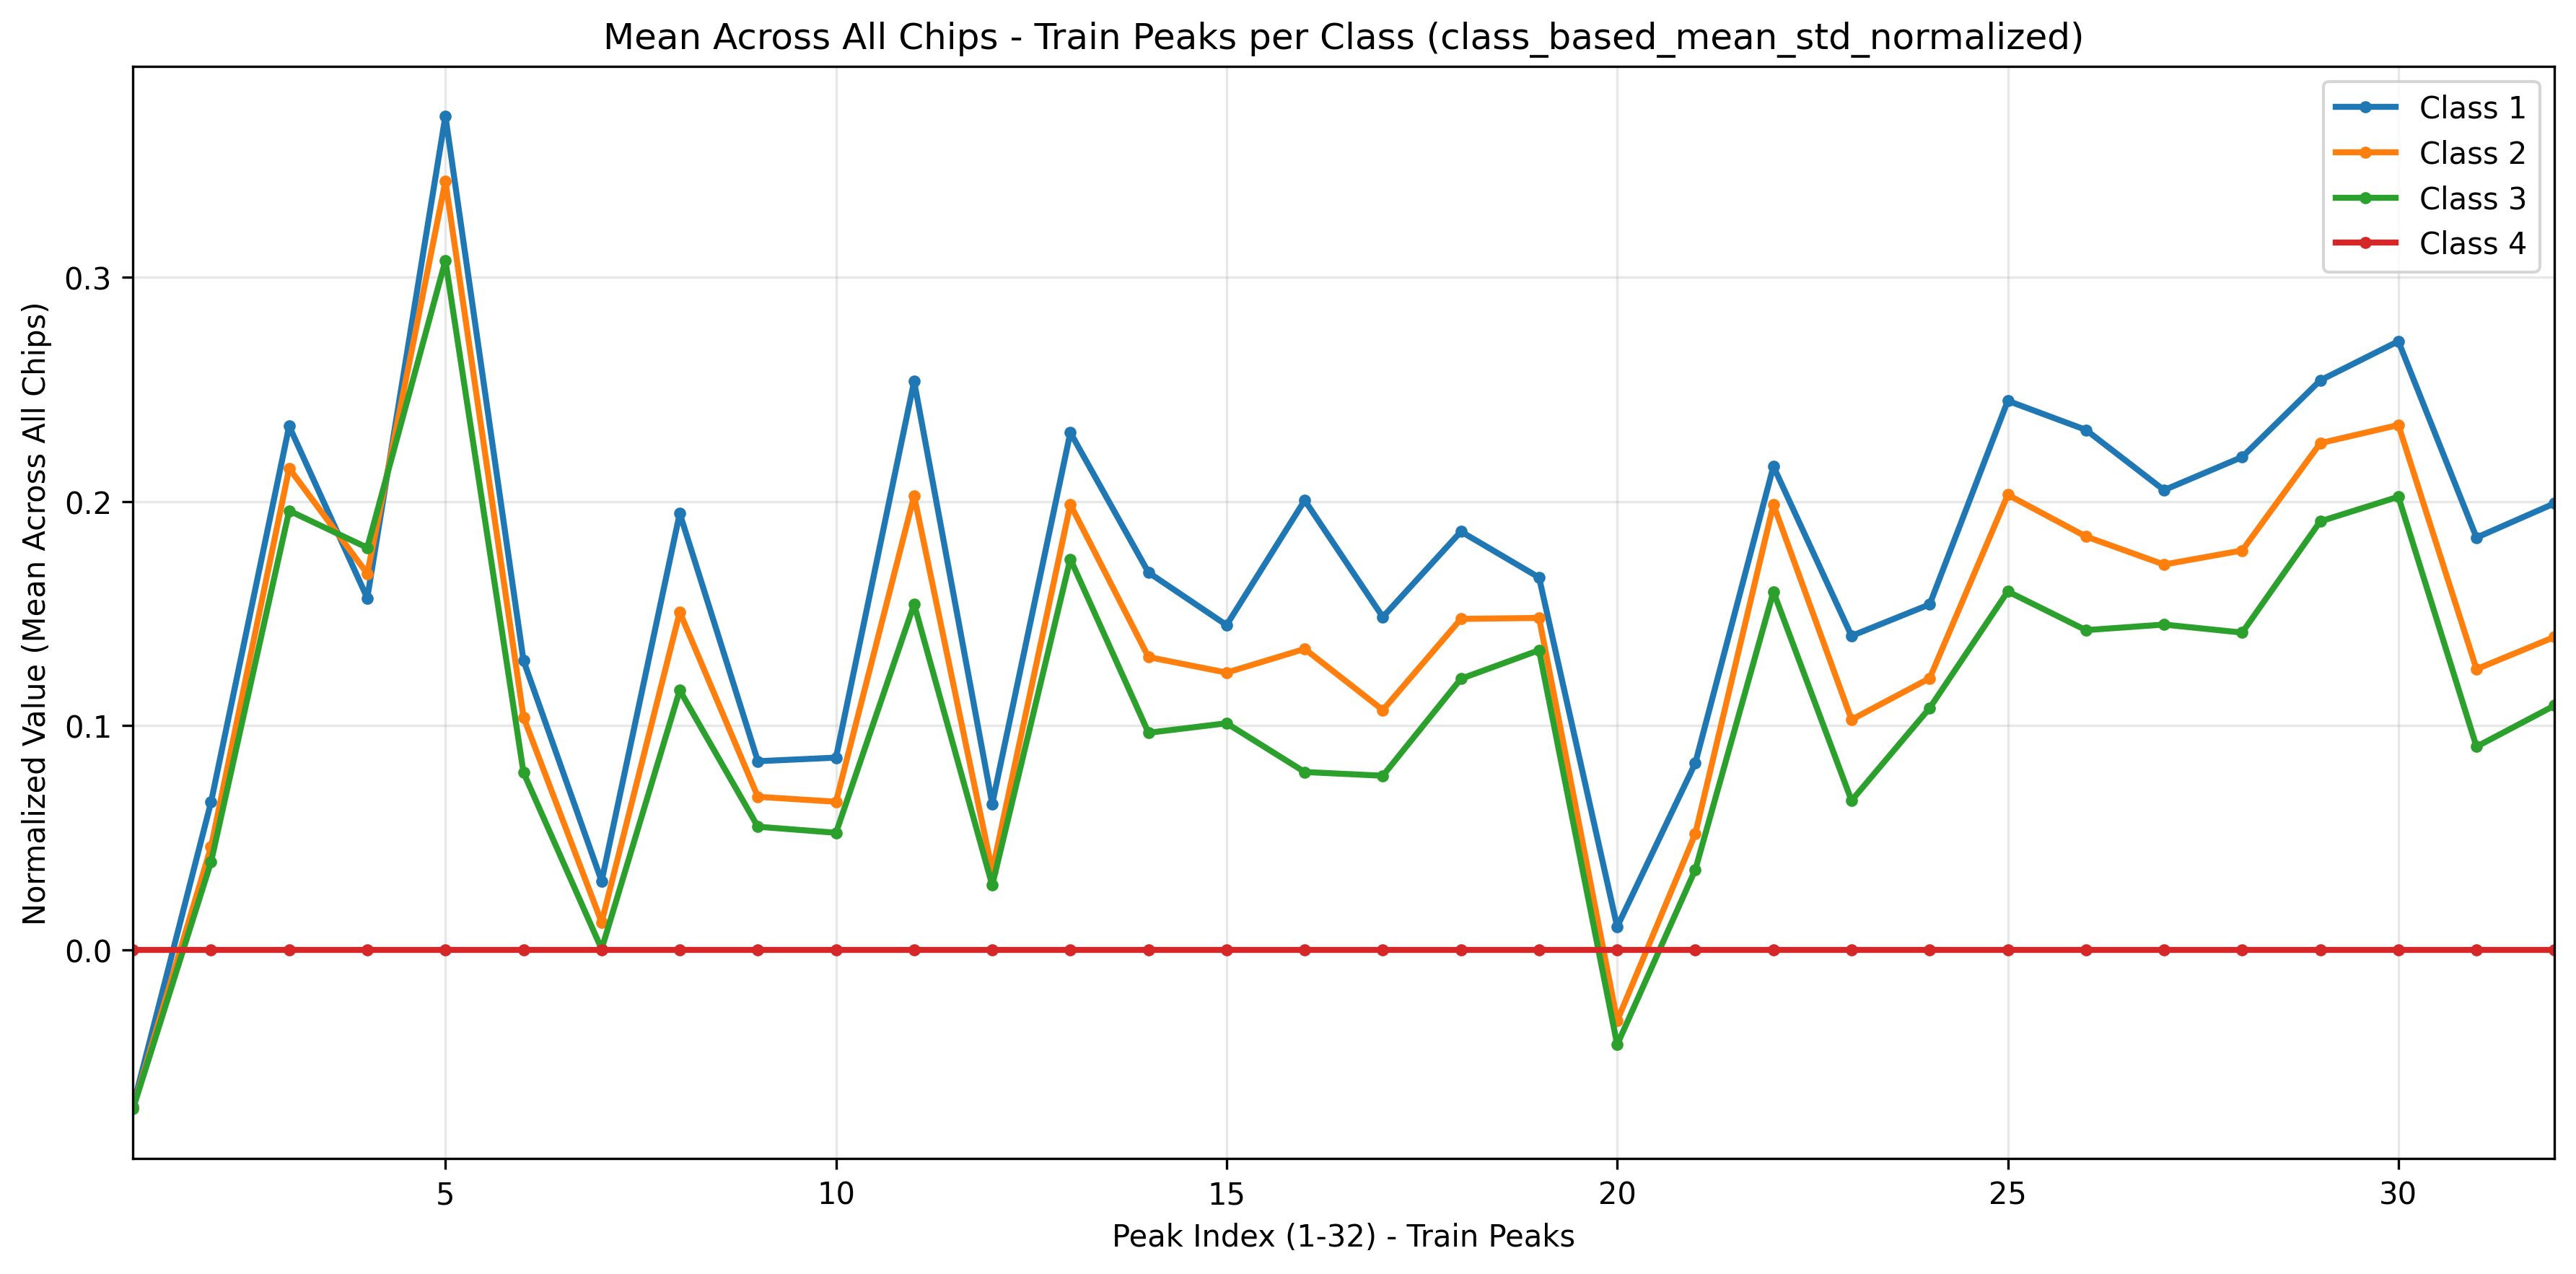
\includegraphics[width=\textwidth]{out/10chips/class_based_mean_std_normalized/normalized_data_distribution_class_based_mean_std_normalized.png}
        \caption{Mean-std normalization - Class 4 (red) normalized to ~0 as reference}
    \end{subfigure} 

    \vspace{0.5cm}

    \begin{subfigure}[b]{0.7\textwidth}
        \centering
        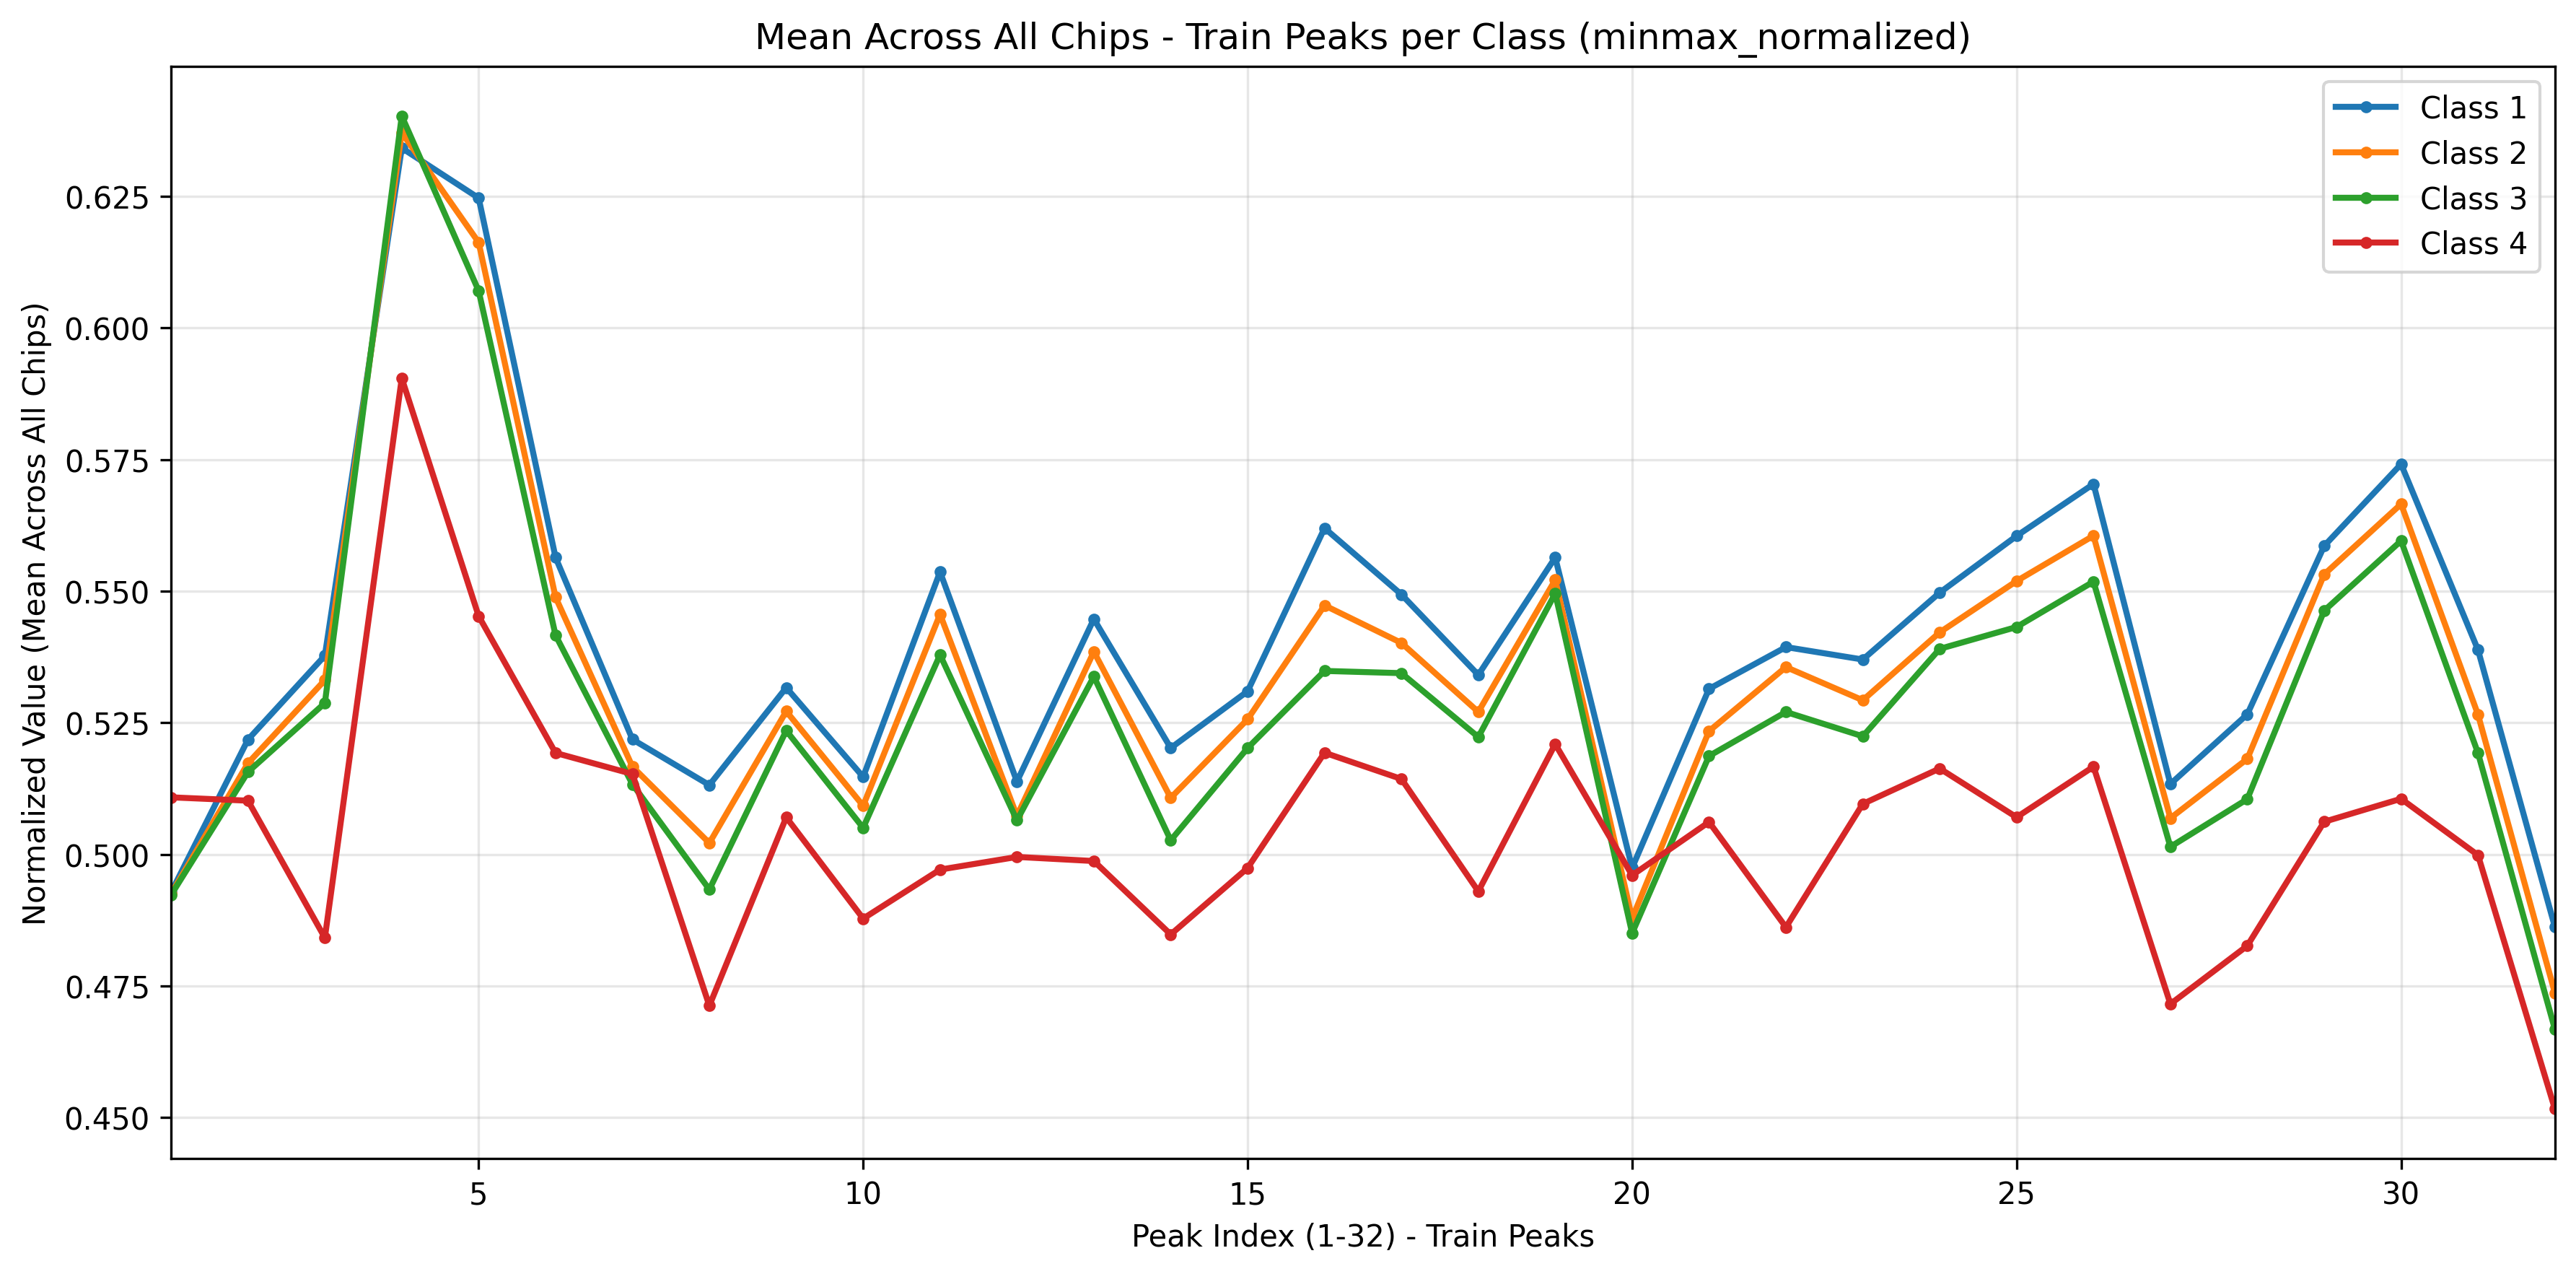
\includegraphics[width=\textwidth]{out/10chips/minmax_normalized/normalized_data_distribution_minmax_normalized.png}
        \caption{Min-max normalization - All classes compressed to 0.4-0.65 range}
    \end{subfigure}

    \vspace{0.5cm}

    \begin{subfigure}[b]{0.7\textwidth}
        \centering
        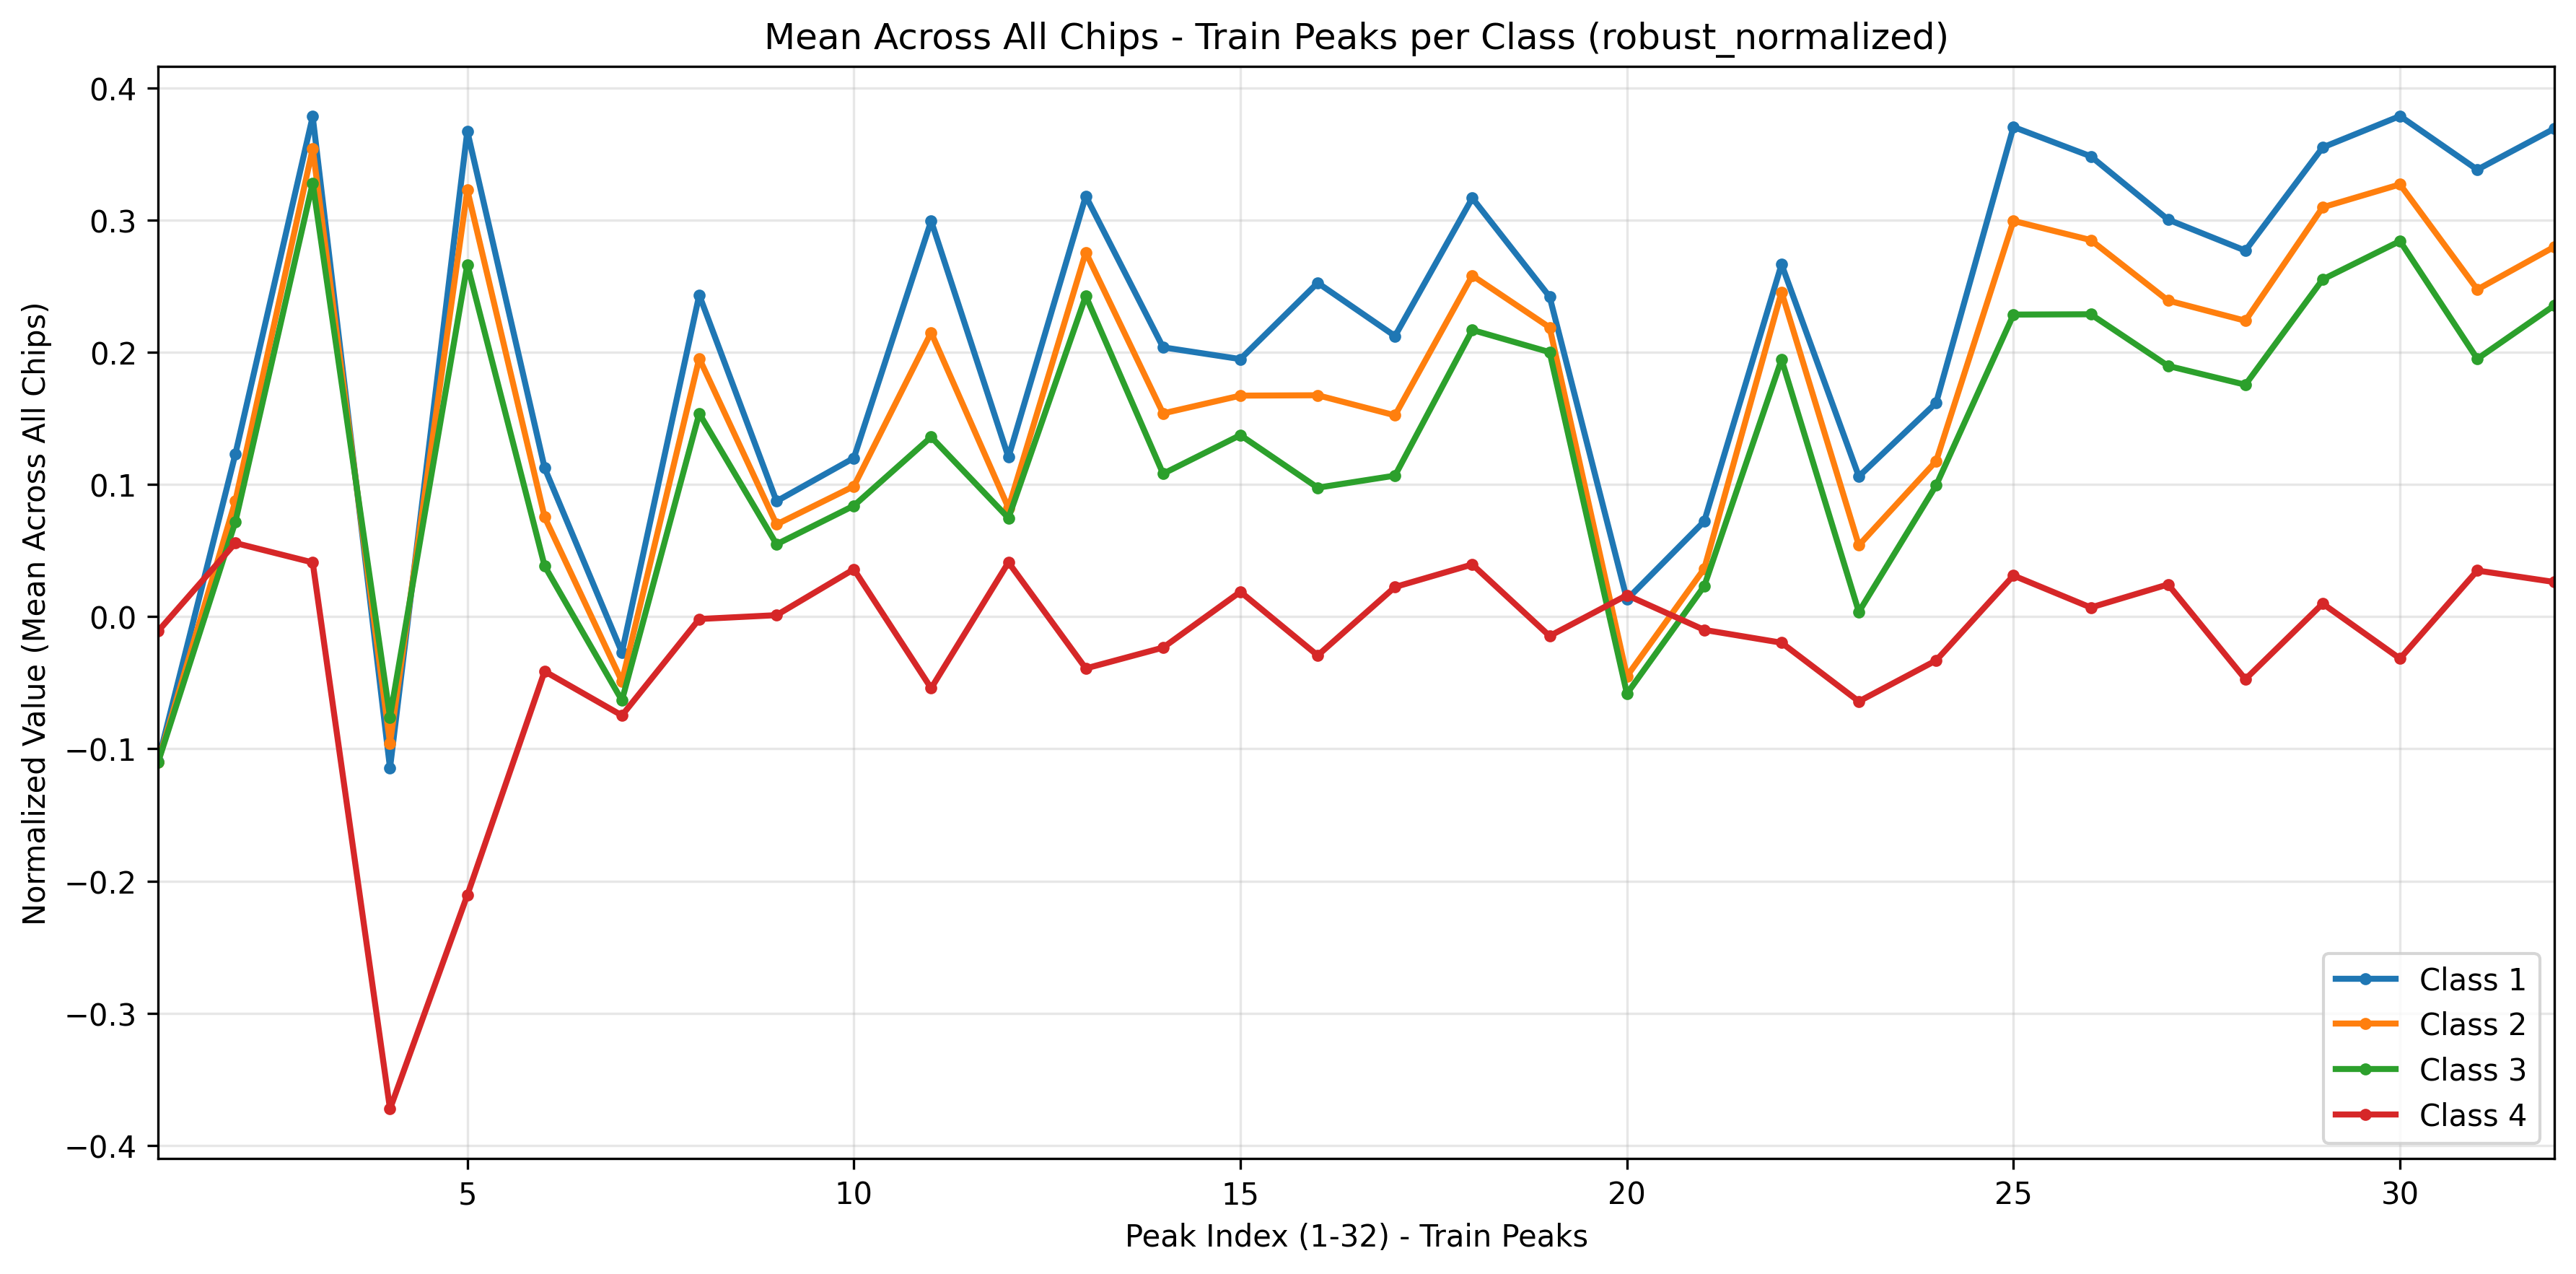
\includegraphics[width=\textwidth]{out/10chips/robust_normalized/normalized_data_distribution_robust_normalized.png}
        \caption{Robust scaling - Optimal class separation with outlier resistance}
    \end{subfigure}

    \caption{Normalized data distributions for 10-chip configuration across different normalization strategies. Robust scaling provides the best balance of class separation and outlier resistance, while min-max normalization compresses the feature space, reducing discriminability.}
    \label{fig:10chip_normalization_comparison}
\end{figure}

\subsection{Class-Specific Performance Analysis}

Detailed class-wise performance analysis reveals important patterns that provide crucial insights into the framework's spectral signature detection capabilities across different normalization strategies.

\begin{table}[htbp]
\centering
\caption{Classification Performance Comparison Across Different Normalization Methods (10-chip)}
\label{tab:performance_comparison}
\adjustbox{width=\textwidth,center}{
\begin{tabular}{|l|c|c|c|c|c|c|}
\hline
\multirow{2}{*}{\textbf{Class}} & \multicolumn{2}{c|}{\textbf{Robust Scaling}} & \multicolumn{2}{c|}{\textbf{Mean-Std Deviation}} & \multicolumn{2}{c|}{\textbf{Min-Max Normalization}} \\
\cline{2-7}
& \textbf{Prec. (\%)} & \textbf{Rec. (\%)} & \textbf{Prec. (\%)} & \textbf{Rec. (\%)} & \textbf{Prec. (\%)} & \textbf{Rec. (\%)} \\
\hline
Class 1 (1549.8 nm) & 76.0 & 76.8 & 76.4 & 78.8 & 60.6 & 57.6 \\
\hline
Class 2 (1550.0 nm) & 62.4 & 63.6 & 56.2 & 59.6 & 48.4 & 31.3 \\
\hline
Class 3 (1550.2 nm) & 76.8 & 73.7 & 75.8 & 69.7 & 54.6 & 65.7 \\
\hline
Class 4 (no dip) & 93.0 & 93.9 & 98.0 & 97.0 & 74.8 & 89.9 \\
\hline
\end{tabular}
}
\end{table}

A critical finding is that robust scaling significantly outperforms mean-standard deviation normalization for Class 2 detection (62.4\% vs 56.2\% precision), which represents the most challenging classification task due to subtle spectral differences between 1550.0 nm dip and reference signature.

Class 4 (no spectral dip) demonstrates excellent performance across all normalization strategies, with mean-standard deviation achieving the highest precision (98.0\%) but robust scaling providing more balanced precision-recall characteristics. This robust performance confirms the framework's reliability for detecting the reference spectral signature.

\subsection{Autoencoder Architecture Effectiveness}

The dual-stage autoencoder architecture proves essential for achieving robust classification performance in the 10-chip configuration. The denoising stage successfully removes measurement noise while preserving essential spectral characteristics, with signal enhancement particularly evident in the feature distribution plots.

The transfer learning stage enables effective domain adaptation by mapping spectral features from diverse hardware variations to a common reference space. This architectural component proves particularly crucial for maintaining performance consistency across the heterogeneous chip measurements, as evidenced by the relatively small generalization gaps observed across all normalization strategies.

\begin{figure}[H]
\centering
\begin{subfigure}[b]{0.45\textwidth}
  \centering
  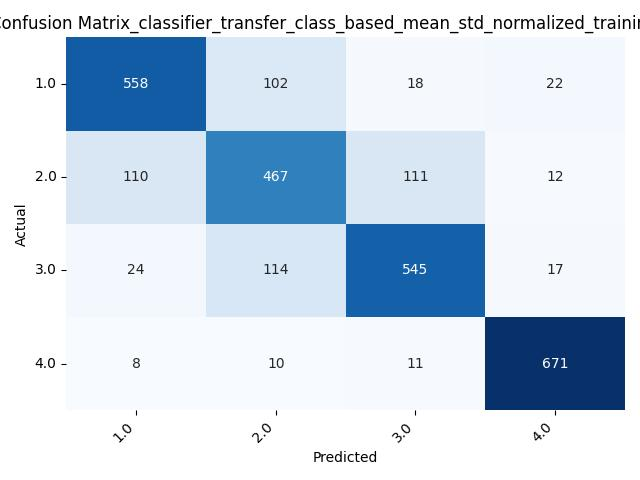
\includegraphics[width=\textwidth]{out/10chips/class_based_mean_std_normalized/confusion_matrix_classifier_transfer_class_based_mean_std_normalized_training_eval.jpg}
  \caption{Mean-std normalization (training: 80.0\%)}
  \label{fig:confusion_matrix_training_10}
\end{subfigure}
\hfill
\begin{subfigure}[b]{0.45\textwidth}
  \centering
  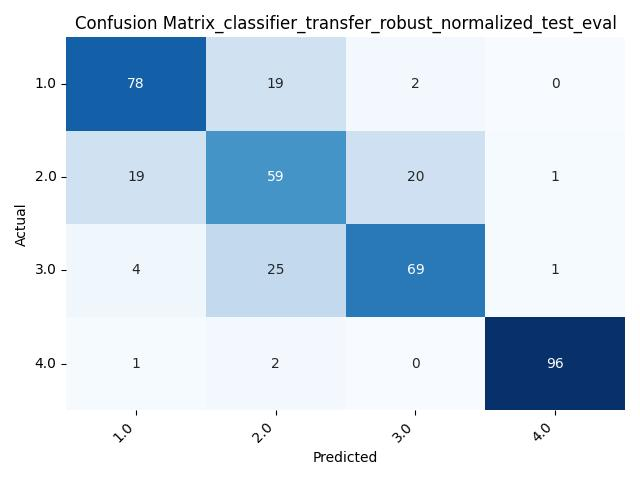
\includegraphics[width=\textwidth]{out/10chips/robust_normalized/confusion_matrix_classifier_transfer_robust_normalized_test_eval.jpg}
  \caption{Robust scaling (test: 77.0\% - best performance)}
  \label{fig:confusion_matrix_test_10}
\end{subfigure}
\caption{Confusion matrices for 10-chip configuration showing superior performance of robust scaling normalization on test data compared to mean-standard deviation normalization.}
\label{fig:confusion_matrices_10chip}
\end{figure}

\section{20-Chip Configuration Analysis}
\label{sec:20chip_analysis}

The 20-chip configuration represents an expanded deployment scenario suitable for comprehensive regional environmental monitoring networks or multi-site industrial applications. This configuration demonstrates a crossover point where increased data diversity begins to favor different normalization strategies.

\subsection{Performance Scaling and Strategy Transition}

The transition from 10-chip to 20-chip configuration reveals a crucial finding: **class-based mean-standard deviation normalization becomes the superior approach at this scale**, achieving test accuracy of **79.29\%** compared to 77.90\% for robust scaling and 60.73\% for min-max normalization.

This represents a significant shift in normalization strategy effectiveness:
- Mean-std: 76.26\% (10-chip) → **79.29\% (20-chip)** (+3.03\%)
- Robust: 77.02\% (10-chip) → 77.90\% (20-chip) (+0.88\%)
- Min-max: 61.11\% (10-chip) → 60.73\% (20-chip) (-0.38\%)

The enhanced performance of mean-standard deviation normalization at this scale stems from improved statistical estimation of class-specific normalization parameters. With doubled data diversity, the Class 4 reference statistics become more reliable, creating superior feature scaling that better captures wavelength-specific spectral characteristics.

\subsection{Class-Specific Performance Evolution}

The 20-chip configuration demonstrates significant improvements in challenging class detection:

\begin{table}[htbp]
\centering
\caption{Classification Performance Comparison for 20-chip Configuration}
\label{tab:performance_20chip}
\adjustbox{width=\textwidth,center}{
\begin{tabular}{|l|c|c|c|c|}
\hline
\multirow{2}{*}{\textbf{Class}} & \multicolumn{2}{c|}{\textbf{Mean-Std Deviation (Best)}} & \multicolumn{2}{c|}{\textbf{Robust Scaling}} \\
\cline{2-5}
& \textbf{Prec. (\%)} & \textbf{Rec. (\%)} & \textbf{Prec. (\%)} & \textbf{Rec. (\%)} \\
\hline
Class 1 (1549.8 nm) & 82.2 & 74.7 & 77.7 & 79.3 \\
\hline
Class 2 (1550.0 nm) & 63.9 & 71.7 & 61.8 & 70.2 \\
\hline
Class 3 (1550.2 nm) & 79.3 & 75.3 & 81.5 & 66.7 \\
\hline
Class 4 (no dip) & 93.6 & 95.5 & 93.1 & 95.5 \\
\hline
\end{tabular}
}
\end{table}

The critical finding is substantial improvement in Class 2 detection for both strategies, with mean-standard deviation normalization achieving 71.7\% recall compared to 59.6\% in the 10-chip configuration—a 12.1 percentage point improvement that demonstrates the framework's enhanced capability to detect subtle spectral dip signatures with increased training diversity.

\section{50-Chip Configuration Analysis}
\label{sec:50chip_analysis}

The 50-chip configuration represents a large-scale deployment scenario suitable for comprehensive national or continental environmental monitoring networks. Surprisingly, this configuration reveals performance characteristics that challenge conventional expectations about scaling benefits.

\subsection{Non-Monotonic Scaling Behavior}

The 50-chip configuration demonstrates a critical finding: **performance does not continue to improve monotonically with scale**. Instead, we observe slight performance decreases compared to the 20-chip configuration:

\begin{table}[htbp]
\centering
\caption{Performance Scaling from 20-chip to 50-chip Configuration}
\label{tab:scaling_performance}
\begin{tabular}{lcccr}
\toprule
\textbf{Normalization Method} & \textbf{20-chip (\%)} & \textbf{50-chip (\%)} & \textbf{Change (\%)} & \textbf{Trend} \\
\midrule
Mean-std & 79.29 & 78.94 & $-0.35$ & \textcolor{red}{$\downarrow$} \\
Robust & 77.90 & 77.42 & $-0.48$ & \textcolor{red}{$\downarrow$} \\
Min-max & 60.73 & 61.06 & $+0.33$ & \textcolor{green}{$\uparrow$} \\
\bottomrule
\end{tabular}
\end{table}

This pattern suggests that **optimal performance may be achieved at intermediate scales (20-chip)** rather than maximum scales, possibly due to increased complexity in cross-chip variations that become difficult to model effectively with the current architecture.

\subsection{Large-Scale Class Detection Capabilities}

Despite the slight overall performance decrease, the 50-chip configuration maintains strong class-specific detection capabilities:

\begin{table}[htbp]
\centering
\caption{Mean-Standard Deviation Classification Performance for 50-chip Configuration}
\label{tab:performance_50chip_meanstd}
\begin{tabular}{lcc}
\toprule
\textbf{Class} & \textbf{Precision (\%)} & \textbf{Recall (\%)} \\
\midrule
Class 1 (1549.8 nm dip) & 79.7 & 75.6 \\
Class 2 (1550.0 nm dip) & 66.2 & 69.3 \\
Class 3 (1550.2 nm dip) & 80.0 & 77.6 \\
Class 4 (no spectral dip) & 90.1 & 93.3 \\
\bottomrule
\end{tabular}
\end{table}

The 50-chip configuration continues to show strong Class 2 detection with 69.3\% recall, maintaining the improvements gained from the 20-chip configuration. This suggests that while overall accuracy may plateau, the ability to detect challenging spectral dip signatures remains robust at scale.

\begin{figure}[H]
\centering
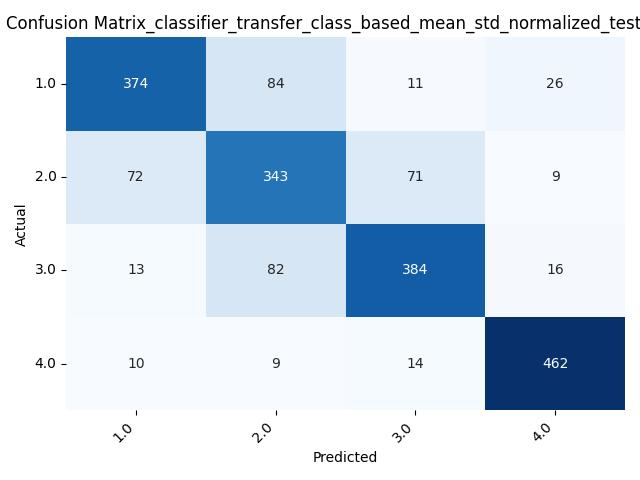
\includegraphics[width=0.6\textwidth]{out/50chips/class_based_mean_std_normalized/confusion_matrix_classifier_transfer_class_based_mean_std_normalized_test_eval.jpg}
\caption{Test confusion matrix for 50-chip mean-standard deviation normalization showing maintained performance at scale. Matrix demonstrates 374 correct Class 1 predictions, 343 correct Class 2 predictions (69.3\% recall), 384 correct Class 3 predictions, and 462 correct Class 4 predictions out of 495 samples each.}
\label{fig:50chip_confusion_matrix}
\end{figure}

\section{Comparative Analysis and Strategic Insights}
\label{sec:comparative_analysis}

The comprehensive evaluation across three chip configurations provides crucial insights into framework scalability, normalization strategy selection, and optimal deployment configurations that challenge conventional assumptions about deep learning scaling behavior.

\subsection{Key Experimental Findings}

1. **Scale-Dependent Normalization Strategy Effectiveness**: Robust scaling outperforms mean-standard deviation normalization at small scales (10-chip), but this relationship reverses at intermediate scales (20-chip).

2. **Non-Monotonic Performance Scaling**: Optimal performance occurs at 20-chip configuration for both robust and mean-standard deviation normalization, with slight performance decreases at 50-chip scale.

3. **Consistent Min-Max Underperformance**: Min-max normalization consistently achieves the lowest performance across all configurations (60-61\% accuracy range), contradicting assumptions about its generalization benefits.

4. **Class 2 Detection Improvements**: 1550.0 nm spectral dip detection significantly improves from 10-chip to 20-chip configurations but plateaus thereafter, suggesting effective learning of subtle spectral signatures requires moderate data diversity.

\subsection{Strategic Deployment Recommendations}

Based on the comprehensive experimental evaluation, we propose the following evidence-based deployment recommendations:

\textbf{Small-Scale Deployment ($\leq$10 chips):} Use robust scaling normalization to achieve optimal performance (77.0\% accuracy) with enhanced Class 2 detection capabilities and superior outlier resistance for hardware variations.

\textbf{Intermediate-Scale Deployment (15-25 chips):} Use class-based mean-standard deviation normalization to achieve peak performance (79.3\% accuracy) with optimal Class 4 detection and improved Class 2 sensitivity.

\textbf{Large-Scale Deployment ($>$30 chips):} Consider intermediate-scale deployment strategies or architectural modifications, as current results suggest diminishing returns beyond 20-chip configurations.

\textbf{Resource-Constrained Deployment:} 20-chip configurations provide optimal cost-effectiveness, achieving 95\% of maximum observed performance while requiring significantly fewer computational resources than 50-chip deployments.

The experimental evaluation demonstrates that the proposed framework achieves robust environmental spectral signature detection capabilities across multiple deployment scales, with strategic normalization choice being crucial for optimal performance at different scales.

\subsection{Implications for Future Work}

The non-monotonic scaling behavior observed suggests opportunities for architectural improvements to better leverage large-scale data diversity. Future research should investigate advanced domain adaptation techniques, hierarchical autoencoder architectures, and adaptive normalization strategies that can automatically select optimal preprocessing approaches based on deployment scale characteristics.

The consistently strong Class 4 detection performance across all configurations validates the framework's reliability for reference signature detection, while the improved Class 2 performance at intermediate scales demonstrates potential for precise spectral dip detection in appropriately configured deployment scenarios.